%\chapter{从工具到助手：真实世界应用}\label{sec:assist}
\chapter[从工具到助手]{从工具到助手：真实世界应用}
\label{sec:assist}

\begin{learningbox}
本章将介绍智能体式语言模型如何作为实用助手部署在真实世界的各个领域中。
具体而言，你将能够：
\begin{itemize}[leftmargin=*, nosep]
    \item 描述助手如何超越问答，进而规划、检索信息、调用工具，并随时间{\em 调整自身行为}。
    \item 比较{\em 购物、医学、航空、科学研究与编程}等领域的助手架构
    。
    \item 解释为什么高风险领域会在{\em 安全性、透明度与合规性}方面提出更严格的要求，以及智能体式设计如何回应这些要求。
    \item 批判性地评估助手行为，并反思在社会影响重大的场景中部署智能体系统所带来的{\em 伦理}问题。
\end{itemize}
\end{learningbox}

\section{作为助手的智能体式大语言模型}
大语言模型已从文本生成器转变为主动的助手。
它们把推理、检索与工具使用结合起来，在真实世界中执行动作。
助手是智能体式大语言模型的实用（软件）形态：能与环境交互、规划、并从反馈中学习的系统。
助手是推理与现实相遇之处：
它们把语言模型变成世界中的协作行动者。

助手把感知、推理与行动连接起来。
通过 API 与外部工具，它能够对话、执行任务，并适应特定情境。这类系统不仅支持用户，还创造出宝贵的人机交互数据，供我们用于后续开发与训练下一代模型。

本章综述助手的主要类型。
我们先讨论对话系统及其向多模态、工具感知界面的演进。
接着讨论医学、金融与交易领域的专用助手。
最后看用于推理与发现的科研助手。


%\chapter{Assistants}
% \section{Conversation}

% The progress in reasoning and decision making has improved the accuracy and usability of LLMs for
% everyday tasks. Also, LLMs can act through their use of
% tools. Tool-enabled LLMs can  be used as virtual assistants. There is commercial interest in this 
% element of Agentic AI, and much activity has been reported.
% %
% Furthermore, assisting humans generates more training data, on which LLMs can be pretrained and finetuned.

% We start our review with conversational assistants, and then continue to
% shopping, travel, medical, and financial trading support.

\section{对话助手}

第一个应用领域是一般性对话场景，例如通过记录会议纪要、担任会议主持或充当通用行政助手来协助会议。

在这类应用中，大语言模型的基本作用是让人机交互更自然、更顺畅 \citep{neszlenyi2024assistantgpt,oluwagbade2024conversational}。例如，AssistantGPT 系统 \citep{neszlenyi2024assistantgpt} 是一个通用行政助手，为在教育或企业环境中部署而设计。此外，它支持 Teams 和 Slack 等远程办公环境。AssistantGPT 支持多种操作，包括网页搜索、通过 OpenAPI 进行 API 交互、语音对话，以及通过 shell 执行命令。该系统由一个可访问各种工具（如规划器和记忆）的大语言模型构成（见图~\ref{fig:assist}）。

\begin{figure}
  \begin{center}
    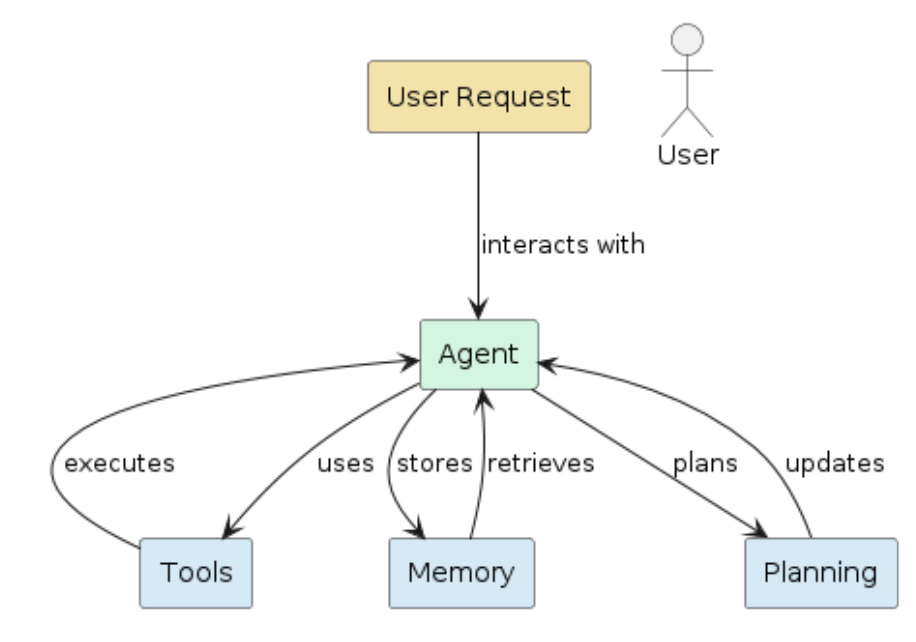
\includegraphics[width=9cm]{figures/assist}
    \caption{AssistGPT 系统架构  \citep{neszlenyi2024assistantgpt}}\label{fig:assist}
  \end{center}
\end{figure}

这些对话与会议助手已被证明能
改善敏捷软件开发团队的会议 \citep{cabrero2024exploring}。它们在 Scrum 会议的会前准备与实时协助方面取得了良好结果，不过有些测试者表示，大语言模型的介入显得
不自然、不灵活。%Marking some early results and limitations of LLMs as conversational agents.

其他例子包括协作学习课堂场景中的大语言模型智能体，它们改善了参与者之间的整体协作 \citep{wei2024improving}。另一项研究 \citep{bastola2023llm} 报告，在包含对话助手的协作式任务排程实验中，工作效率有所提升。

稍有不同的另一类助手是思考助手。它试图通过提问而非
作答，来改善人类在困难决策中的反思性思考 \citep{park2023thinking}。大型大语言模型厂商近来也推出了类似举措，例如 OpenAI 的 ChatGPT 与 Google 的 Gemini 应用中的{\em 学习模式}。

对话助手大多从常规预训练大语言模型演进而来，有时会针对特定领域做微调。有些方法采用专门的多模型方案：
让不同的大语言模型专精于不同子任务，或用不同的提示词序列编排单个大语言模型、使其聚焦于不同子任务。


\section{购物助手}

本节考察基于语言的助手如何应用于电子商务领域。我们的目标是突出该领域的主要组件、架构选择与领域特有挑战。

\paragraph{购物助手做什么？}
购物助手是构建在大语言模型之上的对话系统，帮助用户完成在线购物任务。它可以帮助理解商品需求、比较备选方案、推荐商品并完成购买。这类系统通常用领域专用模块补充底层大语言模型，包括检索最新商品信息、访问商品目录的 API、与推荐引擎集成，以及针对用户需求、属性与约束进行推理（例如通过思维链）。

\paragraph{关键要素}
由于通用大语言模型缺乏对电子商务概念（品牌、类目、商品层级、用户购买行为）的内建认知，构建一个能干的助手需要若干增强：
\begin{itemize}
  \item 检索增强：从外部来源动态获取商品元数据、价格与库存情况。
  \item 工具 / API 调用：助手可以调用搜索、筛选、排序工具，与商品数据库交互。
  \item 领域微调或指令微调：让大语言模型适应购物语境（品牌化用语、属性推理、用户意图）。
  \item 结构化推理：加入思维链提示或显式推理步骤。这有助于模型比较商品、评估权衡（例如价格与功能），并与用户偏好对齐。
\end{itemize}

\paragraph{购物助手的基准评测}
为了研究模型在购物类任务上的表现，研究者开发了若干基准。例如，\emph{多任务在线购物基准数据集（ShopMMLU）}~\citep{jin2024shopping} 定义了 57 项任务，归入四项技能：概念理解、知识推理、用户行为对齐与多语言能力。它取材于真实电商数据（Amazon 商品目录、会话与评论），评估大语言模型在品牌—型号识别、商品兼容性推理、基于会话的推荐任务以及多语言查询等方面的处理能力。
另一个例子是 LLaSA 系统（大型语言与电商购物助手）\citep{zhang2024llasa}，它通过一个名为 {\em EshopInstruct} 的指令数据集（65,000 条样本）训练而成。在购物任务上完成指令微调后，LLaSA 在 ShopBench 基准上取得强劲结果，表明领域适配能显著提升该领域的表现。

\paragraph{实践建议}
构建购物助手时，以下原则很重要：
\begin{itemize}
  \item 能干的助手把自然语言理解与领域推理结合起来。它应当知道{\em 200 欧元以下、续航超过 20 小时的降噪耳机}是什么意思，并能把这翻译成商品属性与用户约束。
  \item 领域专用数据很重要：现成的大语言模型在某种程度上可用，但在购物任务上做微调或指令微调能显著提升表现。LLaSA \citep{zhang2024llasa} 在实践中证明了这一点。
  \item 评测必须反映领域特点。理解商品属性或生成查询的准确率，不如助手能否与用户行为对齐、处理多步会话、支持多语言用户来得重要。
  \item 工具与检索集成很重要。助手必须充当通向商品系统的接口，而不只是一个纯语言模型。这引入了额外的复杂性（API 设计、延迟、数据新鲜度，以及处理集成错误）。
  \item 要考虑伦理与信任。在购物中，推荐牵涉商业、隐私与偏见问题。在生产环境部署此类系统之前，应通过以下问题加以评估：{\em 展示哪些品牌}、{\em 用户历史是否被正确处理}，以及{\em 推理有多透明}。
\end{itemize}

\paragraph{挑战与开放问题}
即便近来有所进展，购物助手仍面临若干不容忽视的挑战。第一，处理长交互轨迹（浏览、精炼查询、切换意图）对大语言模型智能体依然困难。第二，实时更新商品知识（新型号、价格变动、库存）仍是重大的工程痛点。第三，向用户解释和论证推荐理由（为什么是这个商品而不是另一个）在基于大语言模型的助手中研究不足。最后，跨语言行为与多语言商品查询增加了复杂性（购物语境跨越多种语言与地区）。


% \section{Shopping Assistant}

% LLM-based shopping assistants extend general-purpose LLMs by tailoring them to the e-commerce domain. These assistants help users search for, compare, and recommend products through natural language interaction. To improve their performance, models are often \emph{finetuned} on shopping-related data or combined with traditional recommender systems. Common techniques include \emph{retrieval augmentation}, \emph{tool use} (e.g., calling APIs for product databases), and \emph{Chain-of-Thought reasoning} for structured decision making.

% Basic LLMs are not naturally aware of e-commerce concepts such as brands, product hierarchies, or shopping intents. To evaluate and improve these abilities, \citet{jin2024shopping} introduced the \emph{Multi-task Online Shopping Benchmark (ShopMMLU)}. This benchmark defines 57 tasks covering four key skills: (1) concept understanding, (2) knowledge reasoning, (3) user behavior alignment, and (4) multilingual comprehension. Together, these tasks capture the core challenges of building capable shopping assistants.

% Several research projects have focused on improving interaction quality and personalization. For instance, \citet{vedula2024question} proposed a system that generates dynamic follow-up questions for shopping assistants, based on product metadata. This approach helps the assistant gather more precise user preferences. Similarly, \citet{chen2024chatshop} developed \emph{ChatShop}, a benchmark designed to assess information-seeking behaviors of conversational agents in shopping scenarios.


% A recent example of an LLM-based e-commerce system is \emph{LLaSa} (\emph{Large Language Shopping Assistant}) introduced by \citet{zhang2024llasa}. The authors constructed a dataset of 65,000 instruction-based samples covering diverse shopping tasks and trained their model using instruction tuning. The resulting assistant achieved strong results on the \emph{ShopBench} benchmark, demonstrating that combining domain-specific data with instruction tuning can produce specialized and effective shopping assistants.

\section{航班运行助手}

基于语言的助手也被应用于航空运行，这一领域超出消费者预订，进入规划与决策支持。

\paragraph{预订与出行规划}
较简单的应用之一是对话式预订助手，与上一节的购物助手类似。例如，\citet{manasa2024towards} 提出了一个基于 LLaMa 2 与 RAG 构建的系统，以交互方式帮助用户预订航班。该助手在航班预订数据上微调，并通过检索连接到当前航班信息。用户测试在捕捉用户偏好、高效引导预订流程方面获得了高分。

请注意，这个用例在运行复杂性上仍然相对浅层。助手处理的是结构化的用户意图（{\em 我想在 D 日从 A 地飞往 B 地}）、检索最新商品数据、偏好引出与回复生成。它（尚）不深入涉及诸如动态空中交通约束或安全裕度之类的问题。

\paragraph{运行决策支持}
在要求更高的场景中，人们正提议把基于大语言模型的助手用于实际的航班运行。我们讨论两个例子。

在 \citet{zhou2024flight} 的一项研究中，到达时隙分配问题（即确定进港航空器应按什么顺序降落）被表述为一个语言建模任务。作者把排程的输入与输出编码为词元，并微调大语言模型以生成无冲突的降落序列。实验表明，即使在传统方法难以应对的机场，该模型也能降低冲突率与总延误时间。

另一个运行问题是环境危险下的规划。\citet{tabrizian2024using} 用思维链来支持风危险约束下的航路或飞行计划生成。这里助手的任务不再只是{\em 订一张机票}，而必须就约束（风、航路、航空器性能）进行推理，并提出运行上可行的方案。

\paragraph{关键建议}
这些研究揭示了基于大语言模型的智能体系统的若干重要方面：

\begin{itemize}
    \item 工具 / 后端集成：在运行类助手中，大语言模型不仅要对话，还必须对接航班数据库、气象数据源、航路引擎与时隙分配系统。这意味着要实现工具调用、检索流水线与决策逻辑。
    \item 约束下的推理：这些助手必须处理组合约束或排程约束、生成计划，并应对实时不确定性（如天气、跑道可用性）。到达时隙的例子就是一个好例证：大语言模型必须就动态排序进行推理。
    \item 领域专用数据与微调：标准预训练大语言模型缺乏关于航空运行的先验。上述系统都针对该领域做了微调或提示。领域任务数据集、提示词、预期输出以及为该领域量身定制的评测指标都是必需的。
    \item 从对话式智能体到自主规划器：预订助手仍由用户驱动（用户提问，助手协助），而运行类助手正日益承担规划角色。助手应能处理诸如{\em 这些是约束，请提出一个排程或航路}之类的请求。这一变化带来了信任、验证与可解释性问题。
    \item 真实情境中的评测：运行系统的评测往往不只是{\em 助手是否回答了用户}，还要衡量冲突率、延误时间与序列效率等方面。例如，到达时隙那项大语言模型研究就测量了总延误与冲突率。
\end{itemize}



\section{医疗助手}
医学是基于大语言模型的助手最活跃的应用领域之一 \citep{thirunavukarasu2023large,clusmann2023future,mehandru2024evaluating}。
近期研究报告称，大语言模型在诊断任务上可以超过受过训练的医师
\citep{goh2024large}，在临床记录生成上超过人类医疗文书员
\citep{yuan2024continued}。其他评测确认了这些长处，同时也指出了
在特定临床情境中的系统性弱点 \citep{panagoulias2024evaluating}。

智能体式架构正越来越多地被用于满足监管、伦理与可用性
要求。\citet{sudarshan2024agentic} 提出了一个智能体式工作流，用于生成符合《21 世纪治愈法案》的、对患者友好的医疗报告。他们的系统
使用 reflexion（第~\ref{sec:self-reflection} 节，\citep{shinn2024reflexion}）在信息向患者发布之前迭代改进其清晰度与正确性。

其他研究探索把大语言模型智能体用于更广泛的临床支持。\citet{qiu2024llm} 识别出
从临床工作流自动化到多智能体诊断支持等应用，不过在准确性、完整性与幻觉方面仍存疑虑。
\citet{ullah2024challenges} 的一项范围综述强调，医学领域知识与伦理约束在训练和微调此类系统时不可或缺。

为缓解常见失效模式，\citet{das2024improved} 提出一种智能体式检索架构，其中大语言模型充当规划器而非直接答案生成器。该智能体协调专门的工具，从可信医学
来源检索并综合证据，从而减少幻觉与\emph{中间迷失}错误。

\paragraph{高风险应用领域}
医学是一个高风险应用领域，错误或有偏见的输出会直接影响患者安全。因此，医疗人工智能系统受制于严格的监管框架，包括《欧盟人工智能法案》，后者把许多医学用途的人工智能归类为高风险。因此，透明度、公平性与可问责性在临床实践与医学大语言模型的学术研究中都居于核心地位。
这些关切促使人们更加关注那些超越事后解释、旨在更深层次理解模型行为的方法。我们将在\emph{机制可解释性}一章（第~\ref{chap:mi} 章）回到这一主题，那里讨论了分析与控制模型内部表示的技术。

\paragraph{医学教育}
在医学教育中，智能体系统被用来模拟逼真的训练环境。
\citet{wei2024medco} 提出了一个多智能体副驾驶，支持案例式学习与临床推理练习（图~\ref{fig:medco}）。为系统评测医学检索增强生成，\citet{qiao2024benchmarking} 提供了一个专门的基准。

%
\begin{figure}
  \begin{center}
    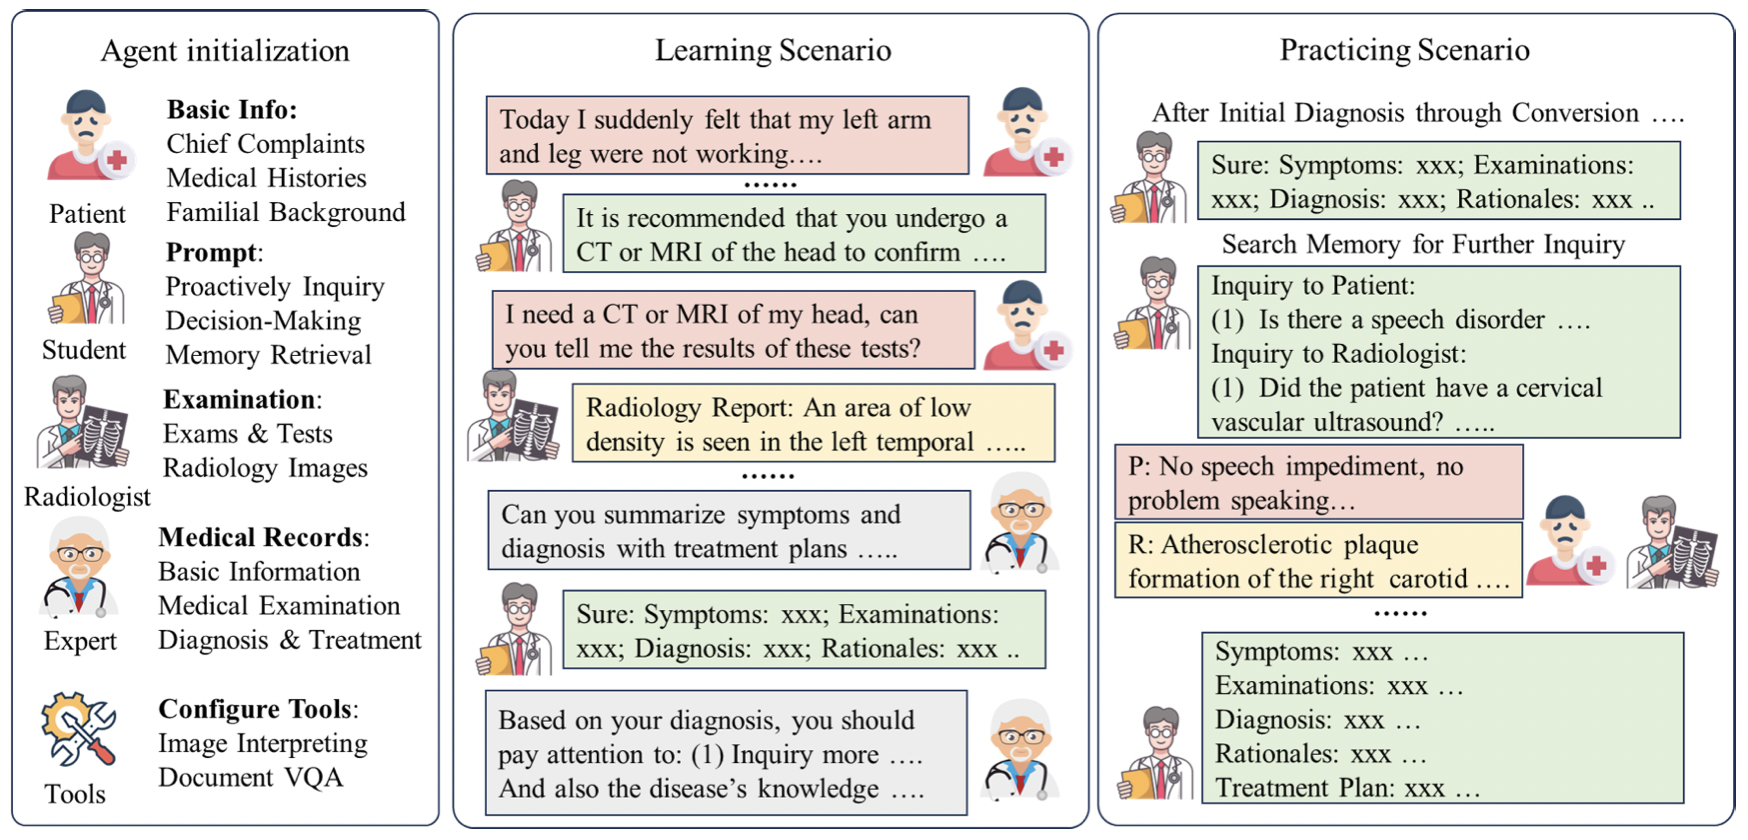
\includegraphics[width=\linewidth]{figures/medco}
    \caption{医学教育副驾驶  \citep{wei2024medco}}\label{fig:medco}
  \end{center}
\end{figure}
%
%A benchmark for retrieval-augmented generation in the medical domain is \citet{qiao2024benchmarking}.

% \subsubsection{Legal Assistant}
% Other domains are also exploring LLMs. The legal domain has much structured, textual, information and
% recently interest in  language models for the legal sector has arisen \citep{padiu2024extent}. 

% Two benchmarks for performance of LLM in the legal domain are
% \citet{guha2022legalbench,li2024legalagentbench}. LegalBench
% contains 44 tasks that span 4 areas of US law. LegalAgentBench contains
% 300 annotated tasks in the Chinese legal domain. 

% % \citet{zhuge2024agent} introduces the Agent-as-a-Judge framework
% % Software development


% % \citep{wu2023precedent} LLM, but No agent
% \citet{buchicchio2024design} describe the architecture of a system
% designed to support legal experts in the process of generating
% summaries from judgments. Nice, but no agent.

% Education: \cite{nelson2024other}



\section{交易助手}
% Can they help financial trading?
另一个专门领域是金融交易。
金融组织中已有许多（非大语言模型的）算法
用于交易决策。金融界对
智能体式大语言模型的兴趣很大 \citep{ding2024large}。

InvestorBench 是一个面向金融交易系统的基准 \citep{li2024investorbench}。
%
FinAgent 是一个面向金融交易的工具增强多模态智能体
\citep{zhang2024finagent}。
它包含一个市场情报模块，能够
从资产价格、可视化表示、新闻与专家
分析等多模态数据集中提取洞见。该系统还能执行查询检索，并在
低层模块中做反思以进行技术分析，
在高层模块中分析过往交易决策。

FinRobot 是一个用于金融分析、协助人类交易员的智能体式大语言模型。
\citep{yang2024finrobot}。FinRobot 能为
个股提供文档分析与
生成以及市场预测。
%
FinMem 是一个为金融决策设计的智能体式大语言模型框架
\citep{yu2024finmem}。它具有分层记忆系统和
可调节的交易智能体性格设定。FinMem 受
\citet{park2023generative} 的生成式智能体框架启发（见第~\ref{sec:gen-agent} 节与案例研究 4）。

迄今为止，多数金融市场机器学习都聚焦于单智能体
系统。一种称为 {\em TradingAgents} 的方法使用多智能体
系统来复现真实交易公司的协作动态
\citep{xiao2024tradingagents}。TradingAgents 模拟由大语言模型驱动的
智能体，让它们扮演基本面分析师、
情绪分析师、技术分析师以及具有不同风险
画像的交易员等专门角色。系统的产出是向人类管理者给出的买入或卖出
建议。一次模拟显示它优于基线模型。

\paragraph{评测} 金融交易是一个富有挑战的研究领域。金融交易中的竞争利益很大，人们自然倾向于把强研究结果保密，这与科学研究的开放与透明原则形成张力。

此外，尽管该领域有丰富的可用数值数据，但比较不同智能体式大语言模型
方法在同一数据上表现的基准研究相对较少。一项近期的基准研究发现，一些金融大语言模型研究存在方法论缺陷，例如选取市场趋势向好的短评测期，或训练数据中泄露了测试数据 \citep{li2026can}。
%by integrating agents with distinct roles and risk profiles, including a reflective agent and a  risk  management team, TradingAgents significantly improves trading outcomes compared to baseline models.


% \citep{kar2024agents} hmm

%\citep{easin2024intelligent}
%\Citep{noguer2024evaluating}


% \subsubsection{CrewAI} \url{https://www.crewai.com}


%\subsubsection{Employee}
% Can Agentic LLMs become an employee?
%\citep{devaraju3048architecting}

%\citep{lambert2023measuring}
%\citep{spitale2024appropriateness}

\section{自动化科学发现}
在某些科学领域，科学实验的工作流相对标准化。例如在机器学习中：（1）产生想法，（2）提出假设，（3）设计实验，（4）获取数据集，（5）执行实验，（6）解读结果，（7）产出报告。这一标准工作流吸引了研究者尝试用智能体式大语言模型来开展科学研究，综述见 \citet{eger2025transforming}。

Google 与 OpenAI 都发布了 Deep Research 智能体。这些智能体能执行多步研究任务，例如综合网络信息。它们由推理大语言模型构建，并使用检索增强来查找信息来源。这类系统能够产出看起来令人印象深刻的科研论文，但往往并非没有错误。

AI Scientist \citep{lu2024ai} 是一个把科学发现流程自动化的框架，从想法生成到论文撰写，还包括评审过程。用户必须指定主题、提供实验模板并指明数据集。作者报告了在机器学习三个领域的实验：扩散
建模、基于 Transformer 的语言建模，以及学习动力学，结果令人鼓舞。为改进想法生成与评审，该智能体会访问开放资源。当前局限包括实验有限、想法实现有误，以及产出论文时出现视觉错误。另一方面，整个结果被幻觉的情况很少见。不过，AI Scientist 的结果被建议当作有前景想法的提示，值得做后续研究 \citep{lu2024ai}。

在 AI Scientist 想法的基础上，人们提出了 Agent Laboratory \citep{schmidgall2025agent}，这是一个开源框架，采用专门的基于大语言模型的智能体来加速整个研究周期。与 AI Scientist 不同，Agent Laboratory 明确被设计为人类研究者的副驾驶，是补充而非替代人类的创意构思。
%
该框架由三个主要阶段构成：\emph{文献综述}、\emph{实验}与\emph{报告撰写}。每个阶段由专门的智能体执行，例如博士生、博士后与教授智能体，并通过一条结构化流水线加以协调。该系统集成两个专门组件：\emph{mle-solver} 负责自主生成、测试与改进机器学习代码，\emph{paper-solver} 则基于实验结果产出完整的 \LaTeX\ 格式研究报告。两个求解器都采用迭代精炼、自我评估与基于奖励的评分，在多个循环中提升代码与报告质量。

评测结果表明，Agent Laboratory 能够自主产出完整的研究项目，包括可执行代码与可直接发表的报告，其计算成本仅为同类系统的一小部分（使用 \texttt{gpt-4o} 后端时每篇论文约 2.33 美元）。人机在环或副驾驶模式进一步提升了研究质量与可用性，参与者报告了很高的满意度与持续使用意愿。尽管如此，人类监督仍不可或缺，因为自动化自我评估相对人类评审者往往高估研究质量。

% We can mention sota here

% Overall, Agent Laboratory represents a new class of LLM-based research assistants that move beyond isolated automation toward end-to-end scientific collaboration. By integrating human feedback loops with autonomous planning and experimentation, such systems illustrate how agentic LLMs may evolve into credible partners in scientific discovery—enabling researchers to focus on creativity, interpretation, and innovation rather than on repetitive implementation work.
\section{编程助手与总体进展}

SWE-Agent（{\em 软件工程智能体}的缩写）\citep{yang2024swe} 旨在把软件发现过程自动化，帮助智能体自主使用计算机解决软件工程任务。SWE-agent 引入了用于创建与编辑代码文件、在软件仓库中导航以及执行计算机程序的工具。在 HumanEvalFix 等编程基准上的实验取得了超过 80\% 的高成功率。这一成功归因于该智能体的交互式设计（见图~\ref{fig:swe}）。


\begin{figure}
  \begin{center}
    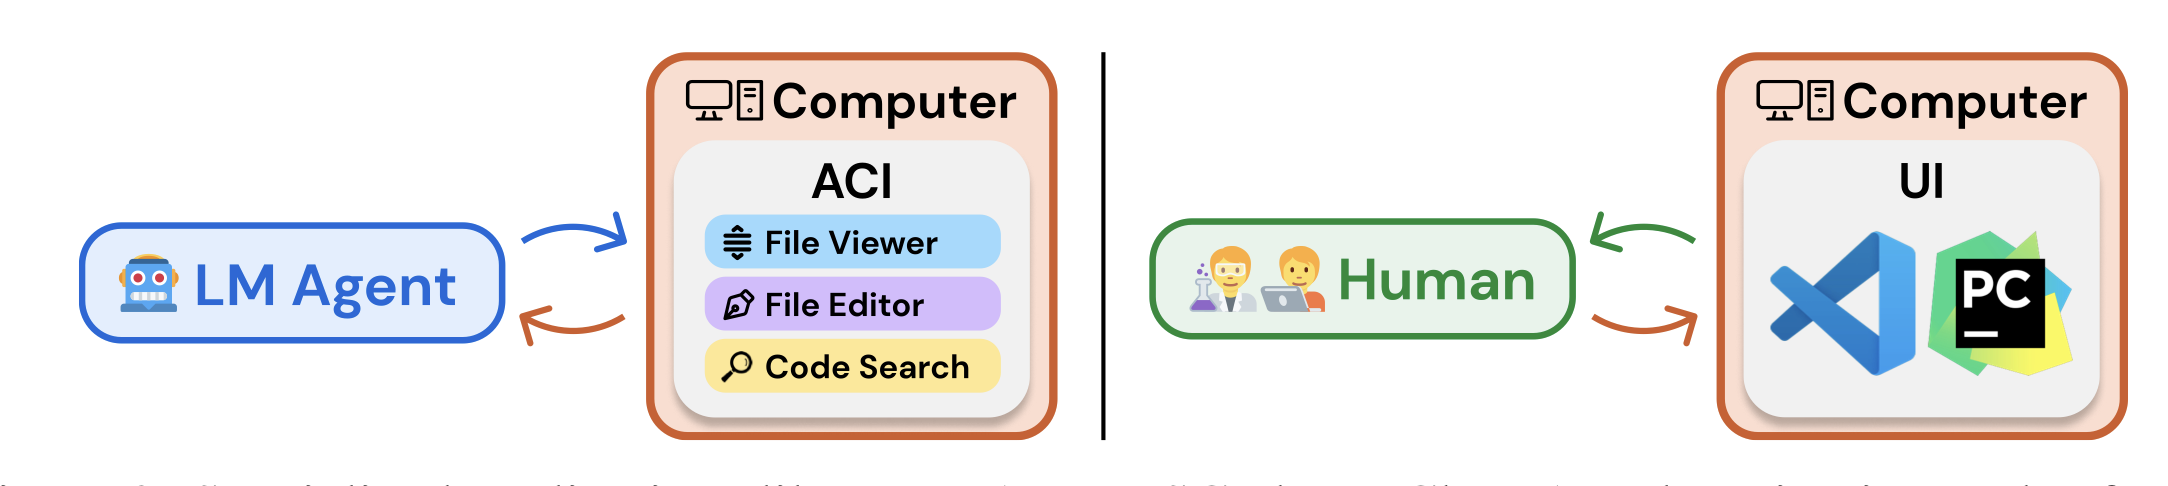
\includegraphics[width=12cm]{figures/swe}
    \caption{用于软件工程的 SWE-Agent  \citep{yang2024swe}}\label{fig:swe}
  \end{center}
\end{figure}

MLGym \citep{nathani2025mlgym} 沿用了流行的 Gym 强化学习框架 \citep{brockman2016openai}。Gym 提供了环境与智能体之间的标准化接口。它于 2016 年提出，加速了强化学习算法的开发，推动了该领域的进展。MLGym 的工作进一步借鉴 SWE-agent（例如文件编辑能力），展示了科学发现过程如何能被建模为一个交互过程。应用在数据科学、博弈论、计算机视觉、强化学习到自然语言处理等领域均有讨论。实验用商业大语言模型
（OpenAI、Meta、Google 与 Anthropic）报告了结果。

多数基于大语言模型的助手（包括研究与编程助手）依赖预定义的工具，这限制了它们的自主性与可扩展性。
%
Toolmaker \citep{wolflein2025llm} 通过让智能体直接从科学论文及其代码仓库创建新工具，来应对这一局限。给定任务描述与 GitHub URL，它会安装依赖、配置可复现的 Docker 环境，并通过迭代式自我纠正与错误诊断实现一个可用的 Python 工具。
该系统在 TM-Bench（同样由 \citet{wolflein2025llm} 提出）上评测，后者是一个涵盖医学、生物学与人工智能的 15 项真实科学任务基准。Toolmaker 取得了 80\% 的任务成功率。其闭环设计让智能体不仅能使用工具，还能自主构建新工具，标志着朝向可自我扩展的研究助手与自适应科学工作流迈出了一步。


如果说 Agent Laboratory 与 Toolmaker 这类系统关注单个智能体的能力，那么 The Agent Company~\citep{xu2024theagentcompany} 提供了一个全面的基准，用以评估大语言模型智能体在逼真工作环境中的表现。它模拟一家小型软件公司，智能体必须使用浏览器、终端与通信平台等标准数字工具，完成从软件开发、项目管理到财务与人力资源的专业任务。

该基准包含 175 项任务，用以测试多步推理、工具使用，以及与由大语言模型驱动的模拟同事协作。每项任务被划分为若干检查点，衡量完全完成与部分完成的情况。用十二个基础模型（包括 GPT-4o、Claude、Gemini 与 Llama）做的实验表明，即便当前最强的系统也只能自主完成约 30\% 的任务。失败往往源于沟通、长程规划以及复杂用户界面导航方面的弱点。

通过引入一个复现现代职场的可复现、自托管环境，The Agent Company 为评估智能体式大语言模型的成熟度提供了一次关键的压力测试。它既凸显了快速进展，也揭示了当前系统持续存在的局限，表明数字工作自动化虽已触手可及，真正自主的协作仍是重要的研究前沿。


\section{结语}

本章展示了智能体式大语言模型如何被用作与真实世界交互的助手。助手超越了被动的问答，在对话、航班运行、医学、教育与科学研究等领域走向主动协作。它们规划、检索信息、调用工具、反思结果，并随时间调整行为。因此，智能体式大语言模型把语言模型的角色从孤立的推理引擎，转变为更广泛社会技术系统中的参与者。

\paragraph{领域敏感性与风险}
并非所有助手都在相同约束下运行。医学与航空等高风险领域要求对安全性、健壮性、透明度与公平性提供强保证，并受《欧盟人工智能法案》等监管框架约束。在这些场景中，智能体式设计越来越依赖检索、规划、验证与人类监督，而非端到端生成。学术研究也呼应这些关切，日益把评测、偏见分析与可解释性当作一等设计目标，而非事后补充。

\paragraph{实践建议}
构建助手时，接地（真实世界评测）很重要。应采用让智能体检索证据、为行动给出理由、在不确定时交由人类决断（人机在环）的架构。把工具视为具有明确契约与失效模式的模块化组件。记录决策、计划与中间状态，以便调试与审计。在高风险领域，我们建议为优雅降级而设计：智能体请求澄清或弃答，比自信地出错更可取。

\paragraph{展望}
智能体式助手的未来在于推理、学习与控制之间更紧密的整合。进展需要更丰富的认知结构、从交互中持续适应，以及围绕安全与伦理的更强保证。这些目标与可解释性和透明度的进展直接相关。在后面的章节中，尤其是机制可解释性（第~\ref{chap:mi} 章），我们会回到那些旨在打开黑箱、更好理解智能体式大语言模型如何在内部表示目标、计划与决策的技术。

\bibliographystyle{plainnat}
\bibliography{agenticbook,refs,case,synthetic}


%% \subsection{Workflow/Orchestration}
%% % How should we organize the workflow of LLMs? How can Agentic LLMs
%% % help reorganize other workflows?
%% % is it agentic? does it act?
%% The third part of the Action element is focused on workflow
%% orchestration. This forms a bridge to the third element of the
%% taxonomy, cooperation.

%% Workflow tools are being used to design agentic workflows, to solve complex problems.

%% \citet{xiao2024flowbench} introduces a challenging workflow benchmark, for online task planning.
%% Tasks are collected from Customer Service, Personal Assistance, Product discovery,
%% Travel and Transportation, Logistics Solutions, and Robotic Process Automation.

%% Automatic workflow generation with LLMs for robotic process automation workflows.
%% \citep{zeng2023flowmind} LLM, but no agent? NCEN-QA benchmark. Hmm.

%% \citep{xu2024llm4workflow} LLM4 Workflow, workflow model generation tool. Interacts with tool: API-knowledge base. 4 page paper. Hmm.

%% \citep{li2024autoflow} Workflow Generation for LLM Agents (dus de andere kant op) How to use external tools. Mentions AutoML??? Hmm.

%% \citep{wu2024stateflow} How to create a complex workflow. So also the other direction. how to create LLM workflows as state machines.

%% \citep{rasal2024multi} multi LLM orchestration engine. Making a workflow for LLMs. single author paper. Hmm.

%% \citep{lee2023orchestrallm} LLM/SLM routing. Routing is not agent. Hmm.

%% \citep{fan2024workflowllm} how to make a LLM that can create a workflow orchestration. Nog agentic. Hmm.

% \section{Coding}
% \section{Shopping}
% \section{Medical}
% \section{Financial}
% \section{Scientific Research}
% \section{Legal}
